\documentclass[border=10pt]{standalone}
\usepackage{tikz}
\usetikzlibrary{arrows.meta}
\tikzset{%
  >={Latex[width=2mm,length=2mm]},
  % Specifications for style of nodes:
            base/.style = {rectangle, rounded corners, draw=black,
                           minimum width=3cm, minimum height=1cm,
                           text centered, font=\sffamily},
       bluebox/.style = {base, fill=blue!15}, %blue!30
       redbox/.style = {base, fill=red!30}, %red
       greenbox/.style = {base, fill=green!30}, %green
       process/.style = {base, minimum width=2.5cm, fill=orange!30, %orange!15
                           font=\ttfamily},
}

\begin{document}
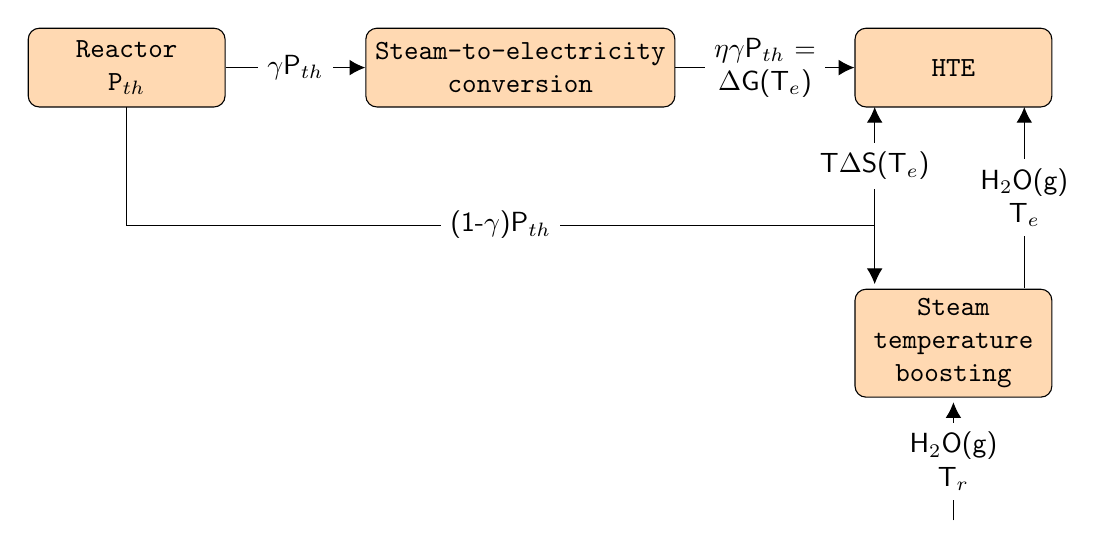
\begin{tikzpicture}[node distance=3cm,
    every node/.style={fill=white, font=\sffamily}, align=center]
  % Specification of nodes (position, etc.)

  \node (reactor)	[process] {Reactor\\P$_{th}$};
  \node (steam1)	[process, right of=reactor, xshift=2.cm] {Steam-to-electricity\\conversion};
  \node (hte)		  [process, right of=steam1, xshift=2.5cm] {HTE};
  \node (steam2)	[process, below of=hte, yshift=-0.5cm, xshift=0.cm] {Steam\\temperature\\boosting};
  
  \draw[->]			(reactor) -- (steam1) node[midway] {$\gamma$P$_{th}$};
  \draw[->]			(reactor) ++(0.,-0.5)-- ++(0.,-1.5)-- node[midway] {(1-$\gamma$)P$_{th}$} ++(9.5,0.)-- node[midway] {T$\Delta$S(T$_e$)} ++(0.,1.5);
  \draw[->]     (hte) ++(-1,-2.)-- ++(0.,-0.75);
  \draw[->]			(steam1) -- (hte) node[midway] {$\eta\gamma$P$_{th}$ =\\ $\Delta$G(T$_e$)};
  
  \draw[->]			(steam2) ++(0,-2.25)-- node[midway] {H$_2$O(g)\\T$_r$} ++(0,1.5);
  \draw[->]			(steam2) ++(0.9,0.7)-- node[midway] {H$_2$O(g)\\T$_e$} ++(0,2.3);

  \end{tikzpicture}
\end{document}